\documentclass{article}
\usepackage[utf8]{inputenc}
\usepackage{graphicx}
\usepackage{tabu}
\usepackage[spanish]{babel}

\begin{document}
\begin{figure}[t!]

\includegraphics[scale=0.3]{logo_udp.PNG}
\label{fig:udplogo}
\end{figure}

\title{\textbf{{Laboratorio 5 \\ STP y VLan 2\vspace{10cm}}}}
\author{\hspace{8cm} Vicente Henriquez \\ \hspace{8cm} Franco Montenegro}
\date{\hspace{8cm} 18/10/2017}

\maketitle
\newpage
\tableofcontents
\newpage
\section{Introducción\vspace{0.5cm}}
En el laboratorio anterior se aprendió sobre las Vlans y a configurar un Switch por medio de Packet Tracer, en este laboratorio lo haremos físicamente a través de nuestros computadores, se asignarán diferentes Vlans a diferentes puertos según lo dictaminado por el ayudante con objeto de aprender lo básico respecto a las herramientas y configuraciones del Switch.
\newpage
\section{Desarrollo\vspace{0.5cm}}
Luego de haber trabajado de forma virtual con un Switch en el laboratorio anterior ahora trabajaremos con dicho dispositivo de manera física, la idea es experimentar con lo aprendido, así que luego de conectar el Switch al PC e instalarlo lo configuraremos a través de Putty, el primer 'experimento' será desactivar el STP y presenciar como se comporta el Switch en tal caso, luego lo reactivaremos y como segundo 'experimento' configuraremos un par de puertos con las VLans que indique el ayudante.\\
Los materiales a utilizar son:
\begin{itemize}
    \item Switch (Figura \ref{fig:Swi})
    \item Cable de Consola (Figura \ref{fig:cabl})
    \item Putty instalado en PC
\end{itemize}
\begin{figure}[h!]
\centering
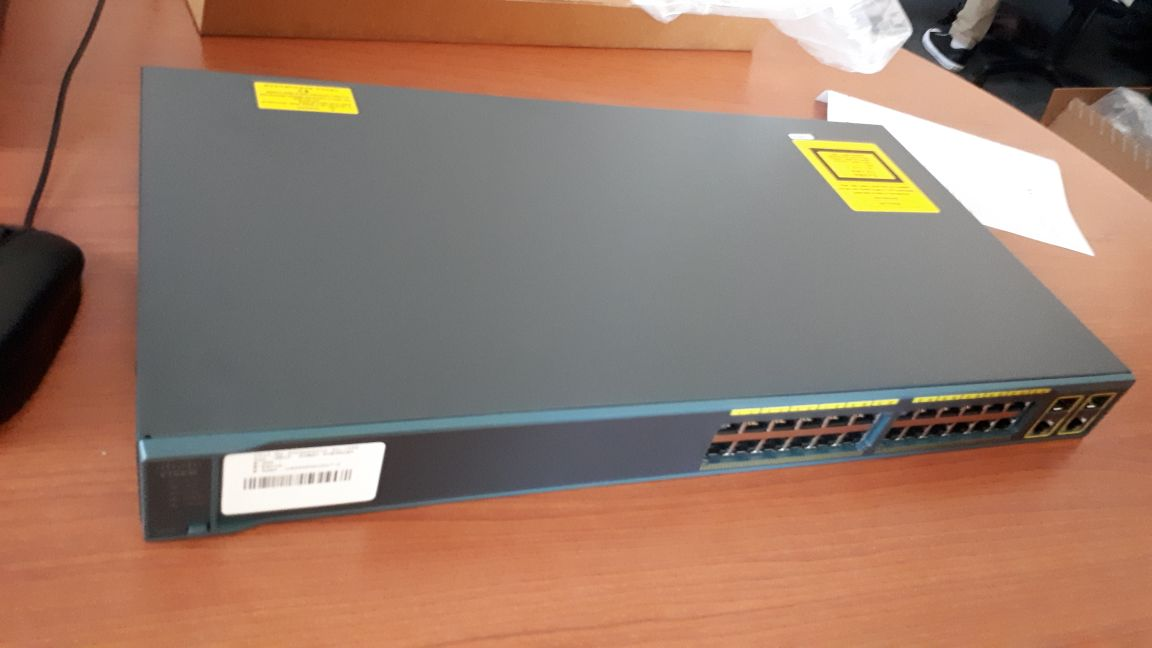
\includegraphics[scale = 0.15]{SwitchDel.jpg}
\caption{Switch}
\label{fig:Swi}
\end{figure}

\begin{figure}[h!]
\centering
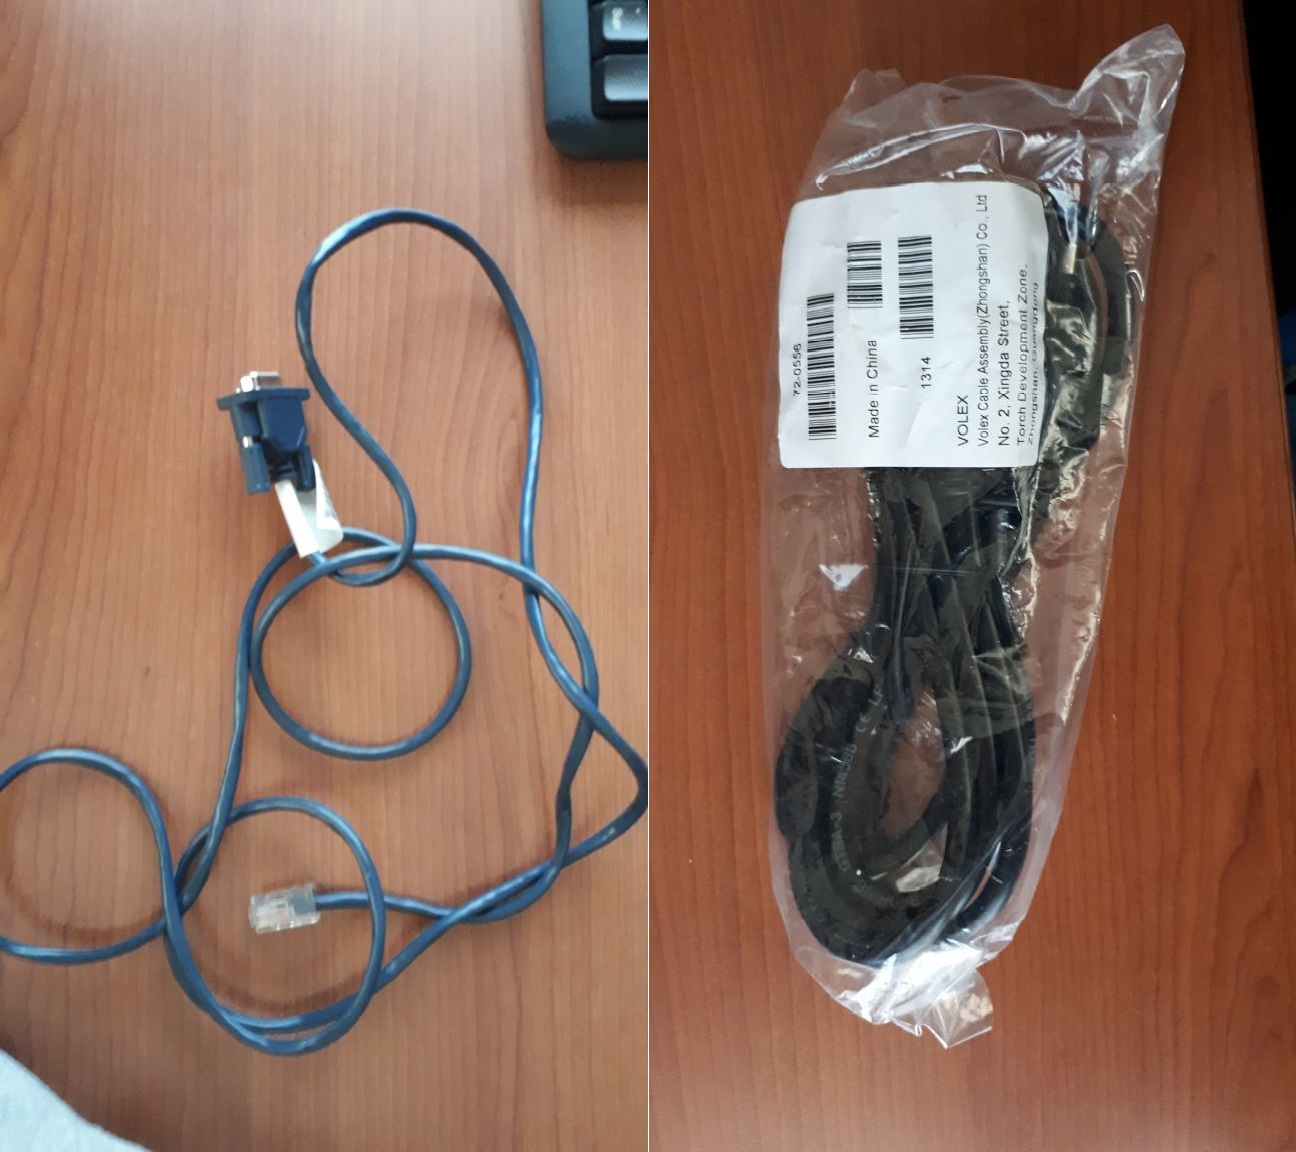
\includegraphics[scale=0.1]{Cables.jpg}
\caption{Cables Consola y Corriente}
\label{fig:cabl}
\end{figure}

\newpage

\begin{figure}[h!]
\centering
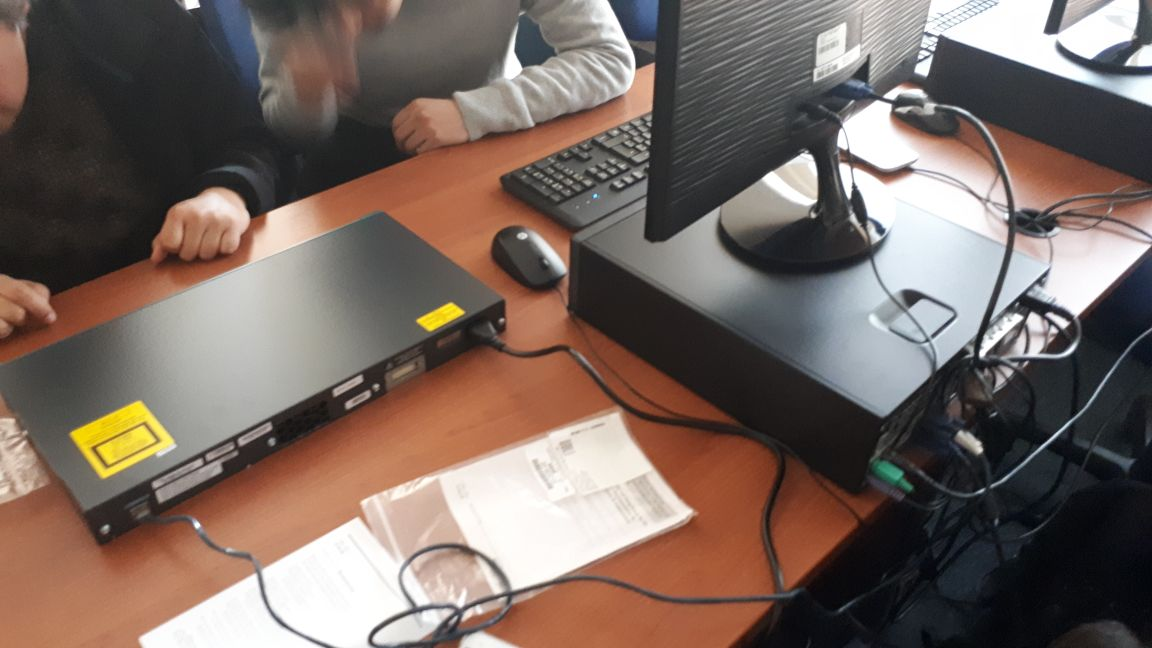
\includegraphics[scale=0.1]{SwitchConectado.jpg}
\caption{Switch Conectado al PC}
\label{fig:conec}
\end{figure}

A continuación y luego de haber conectado el switch al Pc (Figura \ref{fig:conec}), experimentaremos las configuraciones del switch a través de Putty (Figura \ref{fig:inst}).

\begin{figure}[h!]
\centering
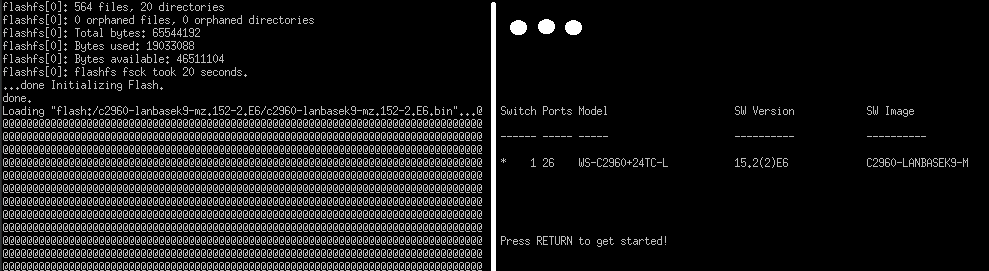
\includegraphics[scale=0.5]{2.png}
\caption{Switch Instalado}
\label{fig:inst}
\end{figure}

Lo primero es desactivar el STP de nuestro Switch (Figura \ref{fig:stpdisable}) y, como ya nos dimos cuenta en el laboratorio anterior, tendremos como resultado una tormenta de broadcast (Figura \ref{fig:tdb}).

\begin{figure}[h!]
\centering
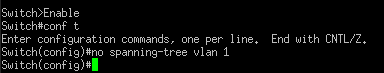
\includegraphics[scale=1]{5_DesactivacionSTP.png}
\caption{STP Desactivado}
\label{fig:stpdisable}
\end{figure}

\begin{figure}[h!]
\centering
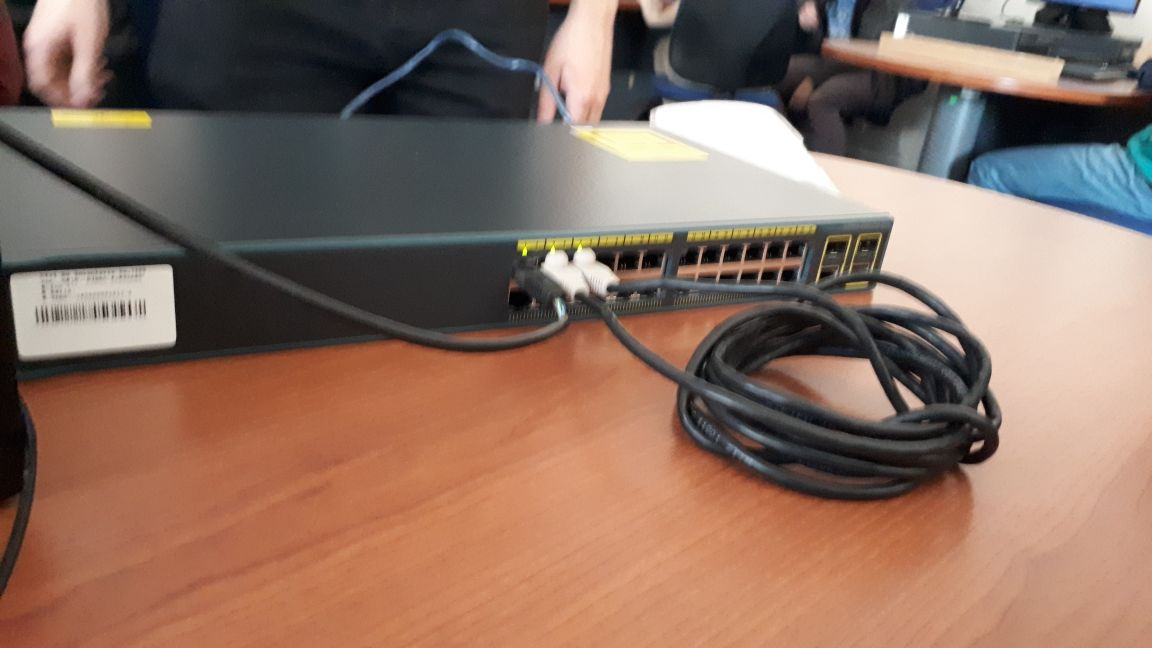
\includegraphics[scale=0.15]{STPdisable.jpg}
\caption{Tormenta de Broadcast}
\label{fig:tdb}
\end{figure}

\newpage
Luego reactivamos el STP y el ayudante nos indica las VLans que debemos crear y a que puertos se las debemos asignar:
\begin{itemize}
    \item Fa 0/1 = VLan 1
    \item Fa 0/2 = VLan 2
    \item Fa 0/3 = VLan 3
    \item Fa 0/4 = Trunk
    \item Fa 0/5 = VLan 1
\end{itemize}
La VLan 1 viene creada por defecto, por lo que se procede a crear las VLans restantes (Figura \ref{fig:CreaV}).
\begin{figure}[h!]
\centering
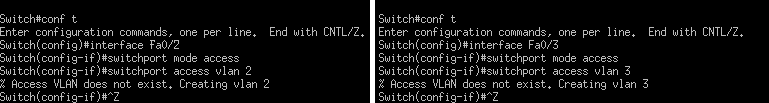
\includegraphics[scale=0.7]{6vlan2y3.png}
\caption{Creación VLan 2 y 3}
\label{fig:CreaV}
\end{figure}

\newline Luego establecemos al puerto Fa 0/4 como Trunk (Figura \ref{fig:SpTrunk}).

\begin{figure}[h!]
\centering
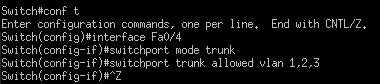
\includegraphics[scale=0.6]{8_vlantrunk4.png}
\caption{Fa 0/4 mode Trunk}
\label{fig:SpTrunk}
\end{figure}

Para terminar de asegurarnos que todo lo hicimos correctamente verificamos los puertos y las VLans(Figura \ref{fig:vlancr}). Posterior a esto se conectó el dispositivo del ayudante a diferentes puertos del switch para reafirmar que todo se hizo bien.
\begin{figure}[h!]
\centering
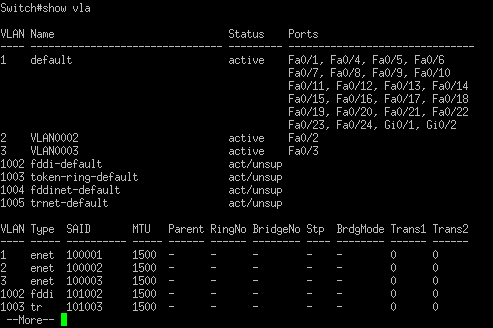
\includegraphics[scale=0.45]{9_vlancreadas.png}
\caption{VLans creadas}
\label{fig:vlancr}
\end{figure}


\newpage
\section{Conclusión\vspace{0.5cm}}
En este laboratorio se reafirma la importancia tanto del STP y de las VLans para las transmisiones y envíos de datos con respecto al laboratorio pasado, ya que sería caótico trabajar sin ellas y esto quedó demostrado en los experimentos realizados.
\end{document}
